\noindent {\it{By S. Boselli, C. M. Carloni Calame, G. Montagna, O. Nicrosini, F. Piccinini, A. Shivaji, F. Yu, Maria Moreno Llacer et al.}}

 We present prospects for studies on {\it CP}-odd couplings in the
 couplings of the Higgs boson with the eletroweak gauge bosons
 as well as in the Yukawa couplings of the Higgs boson with
 fermions, in particular with $\tau^+ \tau^-$ pairs.
 
 \subsubsubsection{\bf CP-odd $VVH$ couplings}

While a large number of studies assessing the impact of {\it CP}-even  
effective operators on Higgs physics is available in the literature 
(see for instance our analysis in Ref.~\cite{Boselli:2017pef} and the references therein), 
the present analysis is focused on the impact of {\it CP}-odd effective operators on the 
interactions among the Higgs boson and the electroweak bosons. 
In the Higgs basis, the CP-violating sector of the BSM Lagrangian affecting $VVH$ couplings 
is given by, 
% 
\begin{eqnarray}
\lag_{\rm CPV} =  \frac{H}{v} \Big[
\tCaa \frac{e^2}{4} A_{\mu\nu}\tilde{A}^{\mu\nu}  
+ \tCza \frac{e\sqrt{g_1^2 + g_2^2}}{2} Z_{\mu\nu}\tilde{A}^{\mu\nu} 
+ \tCzz \frac{g_1^2 + g_2^2}{4} Z_{\mu\nu}\tilde{Z}^{\mu\nu} + \tilde{c}_{WW} \frac{g_2^2}{2}  W^+_{\mu\nu} \tilde W^{-\mu\nu}\Big]
% \left. \vphantom{\half} \rq.
\label{eqn:Hvv}
\end{eqnarray}  
where, $g_1$ and $g_2$ are the $U(1)_Y$  and  $SU(2)_L$ gauge coupling constants. Out of the above four 
parameters only three of them  are independent. In particular,
\begin{equation}
 \tCww = \tCzz + 2s_\theta^2 \tCza + s_\theta^4 \tCaa.
\end{equation}

The processes which are sensitive to CPV operators are the Higgstrahlung processes ($WH$ and $ZH$), the vector boson fusion (VBF) and the Higgs decay into four charged leptons ($H\to4\ell$). Here we focus on angular observables which are sensitive to CPV effects. Indeed, since the total cross-section is a CP-even quantity,  the $1/\Lambda^2$ effects of CPV operators can affect the shape of some specific kinematic distributions only. 



\begin{table*}
	\begin{center}
		\begin{tabular}{lc|cccc}
			\multicolumn{2}{c|}{Process}	 & Combination & Theory & Systematic & Statistical \\ \hline \hline
			\multirow{5}{*}{${H}\to {ZZ}$}   		&$\text{ggF}$& 0.06 & 0.05 & 0.04 & 0.02 \\
			&$\text{VBF}$& 0.17 & 0.10 & 0.10 & 0.10 \\
 			&${WH}$& 0.16 & 0.06 & 0.07 & 0.13 \\
 			&${ZH}$& 0.21 & 0.08 & 0.09 & 0.18 \\ 
 			&${t\overline tH}$& 0.20 & 0.12 & 0.05 & 0.15 \\ \hline
		\end{tabular}
		\caption{Estimated relative uncertainties on the determination of single-Higgs production channels. The 
		estimation of experimental uncertainties is for the high-luminosity LHC (14 TeV center of mass energy and 3 ab$^{-1}$ integrated luminosity)~\cite{}. The theoretical 
		uncertainties are taken from~\cite{}.}\label{tab:one}
	\end{center}
\end{table*}

\subsubsubsection{\bf Global Fit}

To study the sensitive on CP-violating parameters $\tCza$ and $\tCzz$ at HL and HE-LHC, we perform a $\chi^2$ fit using 
the signal strength ($\mu_{i,f}$) as the observable. 
We can build a $\chi^2$  as follows:

\begin{equation}
 \chi^2(\tCza,\tCzz) = \sum_{i,f} \frac{(\mu_{i,f} -\mu_{i,f}^{\rm obs.})^2}{\Delta_{i,f}^2}
\end{equation}
{
The signal strength, $\mu_{i,f}$ is function of the BSM parameters and it is defined as, 
\begin{eqnarray}
 \mu_{i,f} &=& \mu_i \times \mu_f \\
         &=& \frac{\sigma_i^{\rm BSM}}{\sigma_i^{\rm SM}} \times \frac{{\rm BR}_f^{ \rm BSM}}{{\rm BR}_f^{ \rm SM}}.
\end{eqnarray}

The uncertainty, $\Delta_{i,f}^2$ includes theoretical, experimental systematic and statistical uncertainties which 
are added in quadrature to obtain the total uncertainty.
The one-sigma uncertainties for the high-luminosity (14 TeV center of mass energy and 3 ab$^{-1}$ integrated luminosity) are given in table~\ref{tab:one}. 
Assuming same acceptance efficiency, we scale the statistical uncertainties at 14 TeV and 3 ab$^{-1}$ luminosity appropriately 
to obtain the statistical uncertainties at 27 TeV and 15 ab$^{-1}$ 
luminosity. The theoretical and systematic uncertainties are kept unchanged.

When considering kinematic distribution in the fit, we estimate the statistical uncertainty in each bin by scaling 
the overall statistical uncertainty by the fraction of number 
of events in each bin. On the other hand, the theoretical 
and systematic uncertainties are assumed to be the same in all the bins implying 
a very conservative scenario.


Since we are interested in the sensitivity on the CPV parameters that can be reached at HL and HE LHC for which we don't have any data, we take 
$\mu_{i,f}^{\rm obs.}=1$ implying that the future data would be consistent with the SM hypothesis. In the current analysis we consider all the production channels and Higgs decaying to four charged-lepton that is, $i={{\rm ggF, VBF}, ZH, WH, t{\bar t}H}$ and $f=4\ell (2e2\mu, 4e, 4\mu)$. The projected uncertainties in these channels for HL-LHC are given in table~\ref{tab:one}. Note that only the $H\to 4\ell $ decay mode has a non-trivial kinematic distribution and therefore other decay modes in the present analysis have been ignored.
All the results in the following sections are presented taking $M_H=$125 GeV.
}\\

{\bf Production signal strengths : Inclusive} \\

{
The first step is to calculate the signal strengths for the relevant production channels in presence of the CP-violating
parameters $\tCza$ and $\tCzz$. We use MG5~\cite{} to obtain the inclusive cross sections in presence of these parameters. We have generated the required UFO model file for MG5 using the FeynRules package~\cite{}.  At 14 TeV, the production signal strengths are given by, }


\begin{eqnarray}\label{eq:mu14tev}
 \mu_{ZH}^{\rm 14 TeV} &=& 1.00 +  0.54~ \tCza^2 + 2.80~ \tCzz^2 + 0.95~ \tCza \tCzz \\
 \mu_{WH}^{\rm 14 TeV} &=& 1.00  + 0.84~ \tCza^2 + 3.87~ \tCzz^2 
   + 3.63~\tCza\tCzz \\
 \mu_{\rm VBF}^{\rm 14 TeV} &=& 1.00  + 0.25~ \tCza^2 + 0.45~ \tCzz^2  
   + 0.45~\tCza\tCzz
\end{eqnarray}




{ At 27 TeV, the corresponding signal strengths are given by,}

\begin{eqnarray}\label{eq:mu27tev}
 \mu_{ZH}^{\rm 27 TeV} &=& 1.00 +  0.63~ \tCza^2 + 3.26~ \tCzz^2 + 1.11~ \tCza \tCzz \\
 \mu_{WH}^{\rm 27 TeV} &=& 1.00 + 0.98~ \tCza^2 + 4.48~ \tCzz^2 
  + 4.16~\tCza\tCzz \\
 \mu_{\rm VBF}^{\rm 27 TeV} &=& 1.00  + 0.32~ \tCza^2 + 0.67~ \tCzz^2  
  + 0.65~\tCza\tCzz
\end{eqnarray}

The BSM predictions for VBF are derived using following cuts, 
\begin{equation}
 p_T(j) > 20~{\rm GeV}, |\eta(j)| < 5, \Delta\eta_{jj} > 3, m_{jj} > 130~{\rm GeV} \nonumber.
\end{equation}
The $VH$ production modes are more sensitive to $\tCzz$ parameters.
The ggF and $t{\bar t}H$ production channels are unaffected in presence of CP-violating $VVH$ 
couplings. Therefore, 
% 
\begin{eqnarray}
 \mu_{\rm ggF}^{\rm 14 TeV} &=& \mu_{\rm ggF}^{\rm 27 TeV} =  1.00 \\
 \mu_{t \bar t H}^{\rm 14 TeV} &=& \mu_{t\bar t H}^{\rm 27 TeV} =  1.00 .
\end{eqnarray}

{ In the present analysis we do not consider any kinematic distribution in the production channels.} \\

{\bf Decay signal strength : Inclusive} \\


Now we turn to the calculation of signal strength for the decay channel $H \to 4\ell$. This decay 
channel receives contributions from $2e^+2e^-$ ($4e$), $2\mu^+ 2\mu^-$ ($4\mu$) and $e^+e^-\mu^+\mu^-$ ($2e2\mu$) final states.
We use the latest version of the {\tt Hto4l} event generator~\cite{Boselli:2017pef} to obtain the partial decay widths in these 
channels in presence of $\tCza$ and $\tCzz$. Both the $e$ and $\mu$ are treated massless. The ratio of the partial decay widths in BSM and in SM ($R_\Gamma$) for different channels are given by, 

{
\begin{eqnarray}
 R_{\Gamma}(H \to 2e2\mu) &=& 1  + 1.174~ \tCza^2 + 0.00291~ \tCzz^2  
   + (-0.00762)~\tCza\tCzz \\
 R_{\Gamma}(H \to 4e) 
 &=& R_{\Gamma}(H \to 4\mu) \nonumber \\
 &=& 1  + 1.106~ \tCza^2 + 0.00241~ \tCzz^2 
   + (-0.00595)~\tCza\tCzz.
\end{eqnarray}
}
The above expression for Higgs decay 
into $4e$ is obtained after applying a selection cut of { 4 GeV} on the leading and subleading lepton pairs 
of opposite sign.

In the present analysis, we also assume that total Higgs decay width remains unchanged in presence of BSM. In this
case, the signal strength for decay is just the ratio of decay widths in BSM and in SM.
{
\begin{eqnarray}\label{eq:mu4l}
 \mu_{4\ell} &=& \frac{\Gamma^{\rm BSM}_{4\ell}}{\Gamma^{\rm SM}_{4\ell}}  \nn \\
 &=& 1  + 1.138~ \tCza^2 + 
 0.00265~ \tCzz^2  +
 (-0.00674)~ \tCza \tCzz 
\end{eqnarray}
}
We note that, the dependence of the $4\ell$ decay signal strength on the parameter $\tCzz$ is very weak. \\

{\bf Decay signal strength : Differential} \\

{
In our analysis, we are interested in assessing the role of kinematic distributions in $H \to 4\ell$ decay channel 
which are affected by CP-violating $VVH$ couplings, in improving the sensitivity on $\tCza$ and $\tCzz$ at HL and HE-LHC.
% The kinematic variable considered in the present analysis is,
% \begin{equation}
%  	\cos \phi =
% 	\frac{\left( k_{12} \times k_1\right) \cdot \left( k_{12} \times k_3 \right)}
% 	{\left| k_{12} \times k1 \right| \left| k_{12} × k_3 \right|}
% \end{equation}
The Higgs rest frame angle $\phi$ between the decay planes of the two intermediate gauge bosons  
is one of the most sensitive kinematic observables to the CP-Violating $VVH$ couplings. We have considered 50 bins of $\phi$-distribution to perform the fit at differential level. For each bin, we calculate the signal strength ($\mu_{4\ell}^j, j=1\to50$) corresponding 
to Eq.~\ref{eq:mu4l} which is also sensitive to linear terms in $\tCza$ and $\tCzz$.

\subsubsubsection{\bf Result: HL and HE-LHC Analysis}

The results of the $\chi^2$ fit are displayed in Fig.~\ref{fig:fit1p} and Fig.~\ref{fig:fit2p}. In these results, 
 {\it incl.} refers to the fit obtained using 
the total partial decay width information in the $H \to 4\ell$ channel, while {\it diff.} refers to the fit obtained using 
$\phi$-distribution in $H \to 4\ell$ decay. In Fig.~\ref{fig:fit1p}, we show 
$1\sigma$ and $2\sigma$ bounds on $\tCza$ and $\tCzz$ in a one parameter (1P) 
analysis.  At the inclusive level 
we gain better sensitivity on $\tCzz$ than on $\tCza$ when going from HL-LHC 
to HE-LHC. However, due to a stronger dependence of $\mu_{4\ell}$ on $\tCza$ the effect of using $\phi$-distribution in the fit is larger for $\tCza$ than for 
$\tCzz$.

In Fig.~\ref{fig:fit2p}, we provide $1\sigma$ contour lines in the $\tCza-\tCzz$ plane. We can see that the parameters $\tCza$ and $\tCzz$ are weekly correlated. 
Once again we find that using $\phi$-distribution in the fit improves our 
sensitivity on CP-violating parameters significantly.
The parameter $\tCzz$ is mainly constrained by the production channels $VH$ and VBF.
We have given a summary of $1\sigma$ bounds on $\tCza$ and $\tCzz$ obtained from our analysis for HL and HL-LHC in Table~\ref{tab:tab3}.
}



\begin{figure}[h!]
\centering
 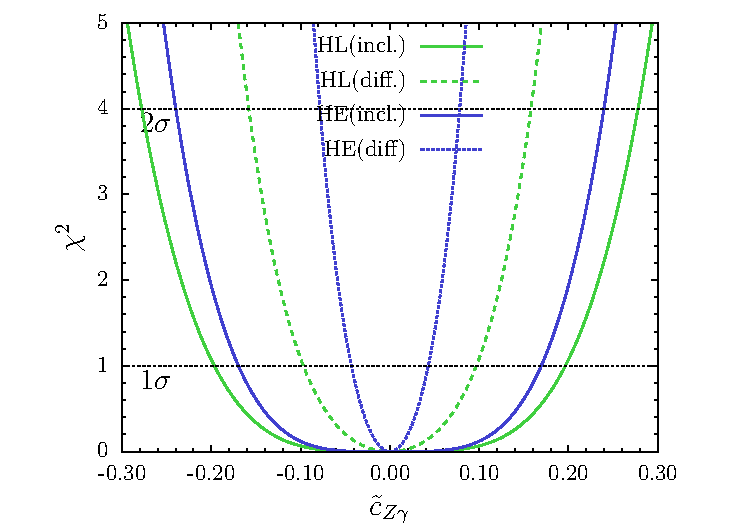
\includegraphics[scale=0.6]{section2/plots/tCza-Chisq-HL3ab-HE15ab}
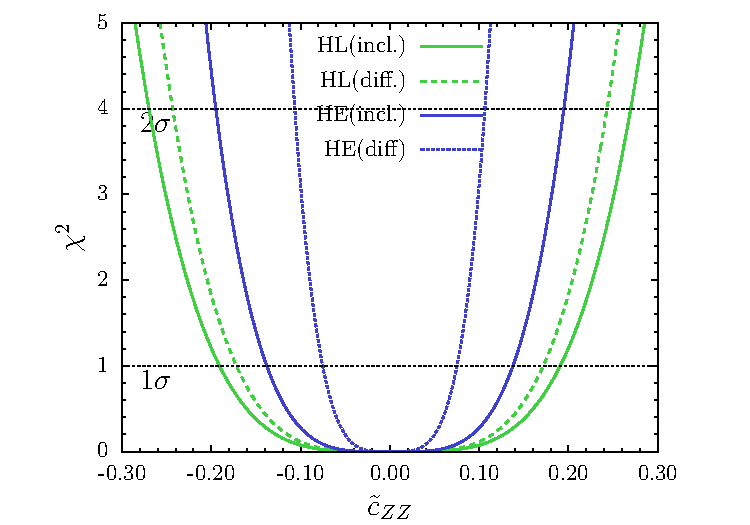
\includegraphics[scale=0.6]{section2/plots/tCzz-Chisq-HL3ab-HE15ab}
\caption{$\chi^2$ dependence on CP-violating parameters taking one parameter non-zero at a time 
at HL (3 ab$^{-1}$) and HE (15 ab$^{-1}$) LHC. {\cred Preliminary} }\label{fig:fit1p}
\end{figure}

\begin{figure}
\centering
 
\includegraphics[scale=1.2]{section2/plots/tCza-tCzz-HL3ab-HE15ab}
\caption{$1\sigma$  reach on $\tCza$ and 
$\tCzz$ at HL (3 ab$^{-1}$) and HE (15 ab$^{-1}$) LHC. {\cred Preliminary} }\label{fig:fit2p}
\end{figure}



\begin{table}
 \centering
 \begin{tabular}{l|cc|l}
 \hline
  \backslashbox{Analysis}{Parameter} & $\tCza$ & $\tCzz$ & Case \\
  \hline\hline
%     8+13 TeV LHC ($4\ell$, incl.) & [-0.30,0.30] & [-0.32,0.32] & 1P \\
%     8+13 TeV LHC ($4\ell$, incl.) & [-0.38,0.38] & [-0.52,0.52] & 1P$_{marg.}$ \\
%     \hline
    HL-LHC ($4\ell$, incl.) & [-0.20,0.20] & [-0.19,0.19]& 1P \\
     HL-LHC ($4\ell$, incl.) & [-0.26,0.26] & [-0.26,0.26]& 1P$_{marg.}$ \\
    \hline
    HL-LHC ($4\ell$, diff.) & [-0.10,0.10] & [-0.17,0.17]& 1P \\
     HL-LHC ($4\ell$, diff.) & [-0.13,0.13] & [-0.22,0.22]& 1P$_{marg.}$ \\
    \hline
    HE-LHC ($4\ell$, incl.) & [-0.17,0.17] & [-0.14,0.14]& 1P \\
     HE-LHC ($4\ell$, incl.) & [-0.22,0.22] & [-0.20,0.20]& 1P$_{marg.}$ \\
    \hline
    HE-LHC ($4\ell$, diff.) & [-0.04,0.04] & [-0.07,0.07]& 1P  \\
     HE-LHC ($4\ell$, diff.) & [-0.06,0.06] & [-0.10,0.10]& 1P$_{marg.}$ \\
 \end{tabular}
\caption{Summary of 1$\sigma$ bounds on $\tCza$ and $\tCzz$ from various analysis considered here. 1P refers to the case
where only one parameter is non-zero while 1P$_{marg.}$ refers to the case in which one of the two parameters is marginalized. {\cred Preliminary}}\label{tab:tab3}
\end{table}




\subsubsubsection{$h \to \tau^+ \tau^-$}

The most promising direct probe of CP violation in fermionic Higgs
decays is the $\tau^+ \tau^-$ decay channel, which benefits from a
relatively large $\tau$ Yukawa giving a SM branching fraction of
$6.3\%$. Measuring the CP violating phase in the tau Yukawa requires a measurement of the linear polarizations of both $\tau$ leptons and and the azimuthal angle between them. This can be done by analyzing tau substructure, namely the angular distribution of the various components of the tau decay products.

The main $\tau$ decay modes studied include $\tau^\pm \to
\rho^\pm (770) \nu$, $\rho^\pm \to \pi^\pm \pi^0$~\cite{Bower:2002zx,
  Desch:2003mw, Desch:2003rw, Harnik:2013aja, Askew:2015mda,
  Jozefowicz:2016kvz} and $\tau^\pm \to \pi^\pm
\nu$~\cite{Berge:2008wi, Berge:2008dr, Berge:2011ij}.  Assuming CPT
symmetry, collider observables for CP violation must be built from
differential distributions based on triple products of three-vectors.
In the first case, $h \to \pi^\pm \pi^0 \pi^\mp \pi^0 \nu \nu$,
angular distributions built only from the outgoing charged and neutral
pions are used to determine the CP properties of the initial $\tau$
Yukawa coupling.  In the second case, $h \to \pi^\pm \pi^\mp \nu \nu$,
there are not enough reconstructible independent momenta to construct an observable sensitive to CP violation, requiring additional kinematic information such as the $\tau$ decay impact parameter.

In the kinematic limit when each outgoing neutrino is taken to be
collinear with its corresponding reconstructed $\rho^\pm$ meson, the
acoplanarity angle, denoted $\Phi$, between the two decay planes
spanned by the $\rho^\pm \to \pi^\pm \pi^0$ decay products is exactly
analogous to the familiar acoplanarity angle from $h \to 4 \ell$
CP-property studies.  Hence, by measuring the $\tau$ decay products in
the single-prong final state, suppressing the irreudicible $Z \to
\tau^+ \tau^-$ and reducible QCD backgrounds, and reconstructing the
acoplanarity angle of $\rho^+$ vs.~$\rho^-$, the differential
distribution in $\Phi$ gives a sinusoidal shape whose maxima and
minima correspond to the CP-phase in the $\tau$ Yukawa coupling.  

An optimal observable using the colinear approximation was derived in~\cite{Harnik:2013aja}. Assuming 70\% efficiency for tagging hadronic $\tau$ final states, and
neglecting detector effects, the estimated sensitivity for the
CP-violating phase of the $\tau$ Yukawa coupling using 3 ab$^{-1}$ at
the HL-LHC is 8.0$^\circ$.  A more sophisticated
analysis~\cite{Askew:2015mda} found that detector resolution effects
on the missing transverse energy distribution degrade the expected
sensitivity considerably, and as such, about 1 ab$^{-1}$ is required
to distinguish a pure scalar coupling (CP phase is zero) from a pure
pseudoscalar coupling (CP phase is $\pi/2$).

At the HE-LHC, the increased signal cross section for Higgs production
is counterbalanced by the increased background rates, and so the main
expectation is that improvements in sensitivity will be driven by the
increased luminosity and more optimized experimental methodology.
Rescaling with the appropriate luminosity factors, the optimistic
sensitivity to the $\tau$ Yukawa phase from acoplanarity studies is
4-5$^\circ$, while the more conservative estimate is roughly an order
of magnitude worse.

\subsubsubsection{$ t\,\bar{t}\,h$}

CP violation in the top quark-Higgs coupling is strongly constrained by EDM measurements and Higgs rate measurements~\cite{Brod:2013cka}. However, these constraints assume that the light quark Yukawa couplings and $hWW$ couplings have their SM values. If this is not the case, the constraints the phase of the top Yukawa coupling relax.
    
Assuming the EDM and Higgs rate  constraints can be avoided, the CP structure of the top quark Yukawa can be probed directly in $pp \to t\bar t h$. Many simple observables, such as $m_{t\bar t h}$ and $p_{T,h}$ are sensitive to the CP structure, but require reconstructing the top quarks and Higgs.

Some $t\bar t h$ observables have been proposed recently that access the CP structure without requiring full event reconstruction. These in include the azimuthal angle between the two leptons in a fully leptonic $t/bar{t}$ decay with the additional requirement that the $p_{T,h} > 200\, \text{GeV}$~\cite{Buckley:2015vsa}, and the angle between the leptons (again in a fully leptonic $t/\bar t$ system) projected onto the plane perpendicular to the $h$ momentum~\cite{Boudjema:2015nda}. These observables only require that the Higgs is reconstructed and are inspired by the sensitivity of $\Delta \phi_{\ell^+\ell^-}$ to top/anti-top spin correlations in $pp \to t\bar t$~\cite{Mahlon:1995zn}. The sensitivity of both of these observables improves at higher Higgs boost (and therefore higher energy), making them promising targets for the HE-LHC, though no dedicated studies have been carried out to date.
